% !TEX root = ../MasterThesis_goto_v1.tex

%%%%%%%%%%%%%%%%%%%%%%%%%%%%%%%%%%%%%%%%%%%%%%%%%%%%%%%%%%%%%%%%%%%%%%%%%%%%%%%%%%%%%%%%%%%%%%%%%%%%%
\chapter{現行の手法との比較} \label{chap:Comparison}

本研究での崩壊点検出の性能の可否についての判断は現行の手法と比較することによって行う。
本章では, そのような比較について議論を行う。
まず\ref{Com:ComparisonwithVF}節では崩壊点検出単体での性能を比較する。

崩壊点検出はジェットの再構成における第一段階である。
したがって, 最終的な性能を知るためには本研究で作成した崩壊点検出を用いたフレーバータギングの性能を確認する必要がある。
このようなフレーバータギングの性能を確認する為, 本崩壊点検出アルゴリズムのLCFIPlusへの導入を行った。
\ref{Com:FlavorTaggingComparison}節ではフレーバータギングを用いたより詳細な比較について述べる。


%%%%%%%%%%%%%%%%%%%%%%%%%%%%%%%%%%%%%%%%%%%%%%%%%%%%%%%%%%%%%%%%%%%%%%%%%%%%%%%%%%%%%%%%%%%%%%%%%%%%%
\section{崩壊点検出単体での比較} \label{Com:ComparisonwithVF}

本研究における崩壊点検出の性能を表\ref{PerformanceofAllEvents}に示した。
表\ref{PerformanceofLCFIPlus}にLCFIPlusで使用されている崩壊点検出の性能である文献\cite{LCFIPlusPaper}の値を示す。
これは本研究の目標値である。
\ref{}項でも述べたように, この評価項目はPrimaryやOthersについては低ければ, BottomやCharmについては高ければ良い性能であるとみなせる。
崩壊点検出での比較では, BottomやCharmの効率が$10\%$以上向上しているとわかる。
一方で, $0.5$より高い閾値を「任意の数の飛跡についてのネットワーク」の出力に設けているが, PrimaryやOthersに関しては性能が悪化してしまっている。
LCFIPlusではBottomやCharmの効率と同一の崩壊チェイン由来の差は$1\%$程度であるのに対し, 本研究の性能では数\%程度の差ができている。
これはLCFIPlusによって再構成されたsecondary vertexは異なる崩壊チェインを跨がずに再構成できているが, 本研究の崩壊点検出は純度が低く異なる崩壊チェインの飛跡を含んでしまっていることを示している。
異なる崩壊チェインを識別するためには崩壊点が生じた方向を再構成する必要があり, ネットワークがそのような崩壊点の位置に関する詳細な情報を再構成できていないためであると考えられる。

崩壊点検出アルゴリズムの性能を一意に決めるのは容易ではないため, より詳細な比較はジェットの再構成の最後段であるフレーバータギングを用いて行うべきである。

\begin{table}[htb]
 \centering
 \small
  \begin{tabular*}{1.0\textwidth}{@{\extracolsep{\fill}}l c c c c}\hline
    真の飛跡の種類 & Primary & Bottom & Charm & Others\\ \hline
    全飛跡の数 & 496897 & 258299 & 247352 & 56432\\
    secondary vertexと判定された飛跡の割合 & 0.6\% & 57.5\% & 64.3\% & 2.5\%\\
    ...同一の崩壊チェイン & - & 56.6\% & 63.4\% & 1.9\%\\
    ...同一の親粒子 & - & 32.2\% & 38.9\% & 1.2\%\\\hline
  \end{tabular*}
  \caption{LCFIPlusでの性能値}
  \label{PerformanceofLCFIPlus}
\end{table}


%%%%%%%%%%%%%%%%%%%%%%%%%%%%%%%%%%%%%%%%%%%%%%%%%%%%%%%%%%%%%%%%%%%%%%%%%%%%%%%%%%%%%%%%%%%%%%%%%%%%%
\section{より詳細な比較} \label{Com:FlavorTaggingComparison}

本研究のネットワークはTensorflowとKerasによって記述されており, それらはPythonを用いて構成されている。
しかしLCFIPlusは前述したようにMarlinのプロセッサーでありC++で記述されているため, LCFIPlus内のフレーバータギングの使用にはPython環境からC++環境への移植が必要である。
本研究ではTensorflow C++ APIを用いて作成したネットワークをC++上で動作させ, 本研究の崩壊点検出アルゴリズムをMarlinプロセッサー実装した。
使用したソフトウェアの環境を次の表\ref{SoftwareEnvironments}にまとめる。
詳細な実装方法については私のGitHubにまとめている\cite{GitHubGotoKLCFIPlus}。

ここではLCFIPlusの崩壊点検出アルゴリズムについてのプロセッサーのみを深層学習を用いたプロセッサーに置き換え, 続くジェットクラスタリング, ジェットバーテックスリファイナー, フレーバータギングについてはLCFIPlusのアルゴリズムを使用する。
したがって, 他のジェット再構成アルゴリズムとの整合性を保つためアルゴリズムに新たな手順を加えた。
その新たな手順について\ref{Com:FlaTagCom:SingleTrackMerge}項で述べる。
また, LCFIPlus内のジェット再構成アルゴリズムについての詳細を再度\ref{Com:FlaTagCom:LCFIPlus}で紹介する。
最後にフレーバータギングの性能について\ref{Com:FlaTagCom:PerformanceofFlavorTagging}項で述べ比較を行う。

\begin{table}[htb]
 \centering
 \small
  \begin{tabular*}{0.75\textwidth}{@{\extracolsep{\fill}}l p{0.375\textwidth}}\hline
    ソフトウェア & バージョン\\\hline\hline
    Bazel & $0.29.1$\\
    Tensorflow C++ API & $2.1.0$\\
    CUDA & $10.1$\\
    cuDNN & $7$\\
    Eigen & $3.3.90$\\
    Protobuf & $3.8$\\
    g++ & $8.4.0$\\
    iLCSoft & $02-02$\\\hline
  \end{tabular*}
  \caption{崩壊点検出のソフトウェア動作環境}
  \label{SoftwareEnvironments}
\end{table}


%%%%%%%%%%%%%%%%%%%%%%%%%%%%%%%%%%%%%%%%%%%%%%%%%%%%%%%%%%%%%%%%%%%%%%%%%%%%%%%%%%%%%%
\subsection{追加のアルゴリズム} \label{Com:FlaTagCom:SingleTrackMerge}

LCFIPlus上で本研究で使用したネットワーク・崩壊点検出アルゴリズムを動作させ次のジェットクラスタリングへその再構成情報を提供する為にアルゴリズムの変更を行った。
現在, LCFIPlusのジェットクラスタリングではLCFIPlusの崩壊点検出によって得られる崩壊点の情報を使用している。
この崩壊点の情報はLCFIPlusのフィッターによって抽出され, それは二本以上の飛跡についての交点を探索するアルゴリズムである。
しかし, 本研究の崩壊点検出アルゴリズムではその性質上, 飛跡が一本しか含まれていないsecondary vertexが生成されてしまう場合がある。
LCFIPlusのジェットクラスタリングを使用するに当たって, LCFIPlusのフィッターで得られる崩壊点の情報は必須である為, 本研究の崩壊点検出アルゴリズムにおいても飛跡を一本しか含まない崩壊点を他の崩壊点に統合しなければならない。

ここでは, その様な崩壊点の飛跡とその他のsecondary vertex内の全ての飛跡について, 飛跡対を作りLCFIPlusのフィッターによって最も$\chi^2$の小さくなる飛跡対の組み合わせを選び, 飛跡を一本しか含まない崩壊点を選ばれた飛跡を含む崩壊点に統合した。
これを飛跡一本の崩壊点が無くなるまで繰り返し, 全てのsecondary vertexが二本以上の飛跡を持つ様に修正した。
その様にして再構成された崩壊点について, LCFIPlusのフィッターによって崩壊点の情報を抽出する。

以上より崩壊点の生成を深層学習を用いて行い, 崩壊点の情報をLCFIPlusのフィッターによって得るプロセッサーを作成し, 現行の崩壊点検出と本研究の崩壊点検出を入れ替えたジェットの再構成を行う。
崩壊点検出以降のLCFIPlusのアルゴリズムについて次の\ref{Com:FlaTagCom:LCFIPlus}項でまとめる。


%%%%%%%%%%%%%%%%%%%%%%%%%%%%%%%%%%%%%%%%%%%%%%%%%%%%%%%%%%%%%%%%%%%%%%%%%%%%%%%%%%%%%%
\subsection{LCFIPlus} \label{Com:FlaTagCom:LCFIPlus}

LCFIPlusのジェットクラスタリングは崩壊点検出によって得られた崩壊点の情報を使用して中性電荷の飛跡を含めた全ての飛跡についてクラスタリングを行う。
LCFIPlusではこのジェットクラスタリングの前に重いハドロン粒子のセミレプトニック崩壊によって生じた孤立レプトンの探索を行う。
ここではエネルギーや衝突係数を用いて判定する。
次に得られた孤立レプトンとsecondary vertexの組み合わせを行う。
LCFIPlusでは孤立レプトンについては運動量方向を, secondary vertexについてはprimary vertexからの角度を用いそれらの開き角が一定以下であるかによって評価している。
これらの手順により再構成された孤立レプトンや崩壊点はジェットクラスタリングのコアとして使用される。
ジェットクラスタリングはDurhamアルゴリズムを用いており, 粒子の運動量方向とジェットに開き角, 修正Durham距離に基づいてジェットの再構成を行っている。

LCFIPlusではボトム・フレーバーのジェットとチャーム・フレーバーのジェットをより精度よく区別するためにジェットバーテックスリファイナーアルゴリズムが使用されている。
ジェットバーテックスリファイナーはシングルトラック崩壊点検出と崩壊点コンバイナの二つのステップで行われる。
シングルトラック崩壊点検出では崩壊点を一つしか含まないジェットについて, 飛跡を一本だけ含む疑似崩壊点を探索するアルゴリズムである。
崩壊点コンバイナは二つ以上の崩壊点を含むジェットについて崩壊点の個数を最大二つに結合させるアルゴリズムである。
再構成された崩壊点について更に一つに纏められる場合は新たな崩壊点に置き換え, また二つの崩壊点の距離を用いて崩壊点の選択を行う。

\ref{Intro:SoftERILC:JetReconstruction}項でも述べた様にLCFIPlusのフレーバータギングはBDTsを用いて行われる。
BDTsはROOTのTMVAパッケージを使用し, ボトム・フレーバーのジェット, チャーム・フレーバーのジェット, アップ, ダウン, ストレンジ・フレーバーのジェットの三つにクラスで分類している。
入力変数はジェット内の崩壊点や飛跡などの構成要素によって作成され, ジェットのエネルギーに依存する様な変数については規格化を行っている。

以上が崩壊点検出以外のLCFIPlus内のアルゴリズムである。
本研究では深層学習を用いた崩壊点検出によってsecondary vettexの探索を行い, その後にこれらのアルゴリズムを使用することで, フレーバータギングの性能を評価する。


%%%%%%%%%%%%%%%%%%%%%%%%%%%%%%%%%%%%%%%%%%%%%%%%%%%%%%%%%%%%%%%%%%%%%%%%%%%%%%%%%%%%%%%%%%%%%%%%%%%%%
\subsection{本研究の崩壊点検出を用いたジェット再構成の性能} \label{Com:FlaTagCom:PerformanceofFlavorTagging}

まず, ジェットバーテックスリファイナーアルゴリズムによって再構成された崩壊点と疑似崩壊点の情報を表\ref{TheNumberofReconstructedVertices}にまとめる。
括弧内はLCFIPlusの性能との相対値である。

\begin{table}[htb]
 \centering
 \small
  \begin{tabular}{l l l l}\hline
    (崩壊点, 疑似崩壊点) & ボトム & チャーム & アップ, ダウン, ストレンジ\\\hline\hline
    (0, 0) & 12.7\% (-8.6) & 49.1\% (-10.2) & 93.8\% (-4.3)\\
    (0, 1) & 1.25\% (-0.36) & 0.41\% (-2.4) & 0.10\% (0.9)\\
    (1, 0) & 47.9\% (10.2) & 48.1\% (8.3) & 5.96\% (4.16)\\
    (1, 1) & 9.41\% (-4.1) & 0.90\% (0.36) & 0.03\% (0.01)\\
    (2, 0) & 28.7\% (4.9) & 1.46\% (1.27) & 0.07\% (0.03)\\\hline
  \end{tabular}
  \caption{再構成された崩壊点と疑似崩壊点の個数}
  \label{TheNumberofReconstructedVertices}
\end{table}

LCFIPlusと比較して本研究の崩壊点検出は疑似崩壊点ではなく崩壊点による項目の値が大きくなっており, 崩壊点検出がより多くの崩壊点の候補を探索しているとわかる。
また, アップ, ダウン, ストレンジ・フレーバーのジェットに関しても崩壊点を探索してしまっており, ノイズとなってしまっている可能性がある。

フレーバータギングの性能はROC曲線を用いた評価を行う。
ここではボトム・ジェットについての効率とチャーム・ジェットについての効率についてそれぞれROC曲線を描画した。
図\ref{5-2-3-1FlavorTaggingROCCurve}では横軸に信号効率, 縦軸にログスケールの背景効率を示している。

\begin{figure}[htbp]
 \centering
 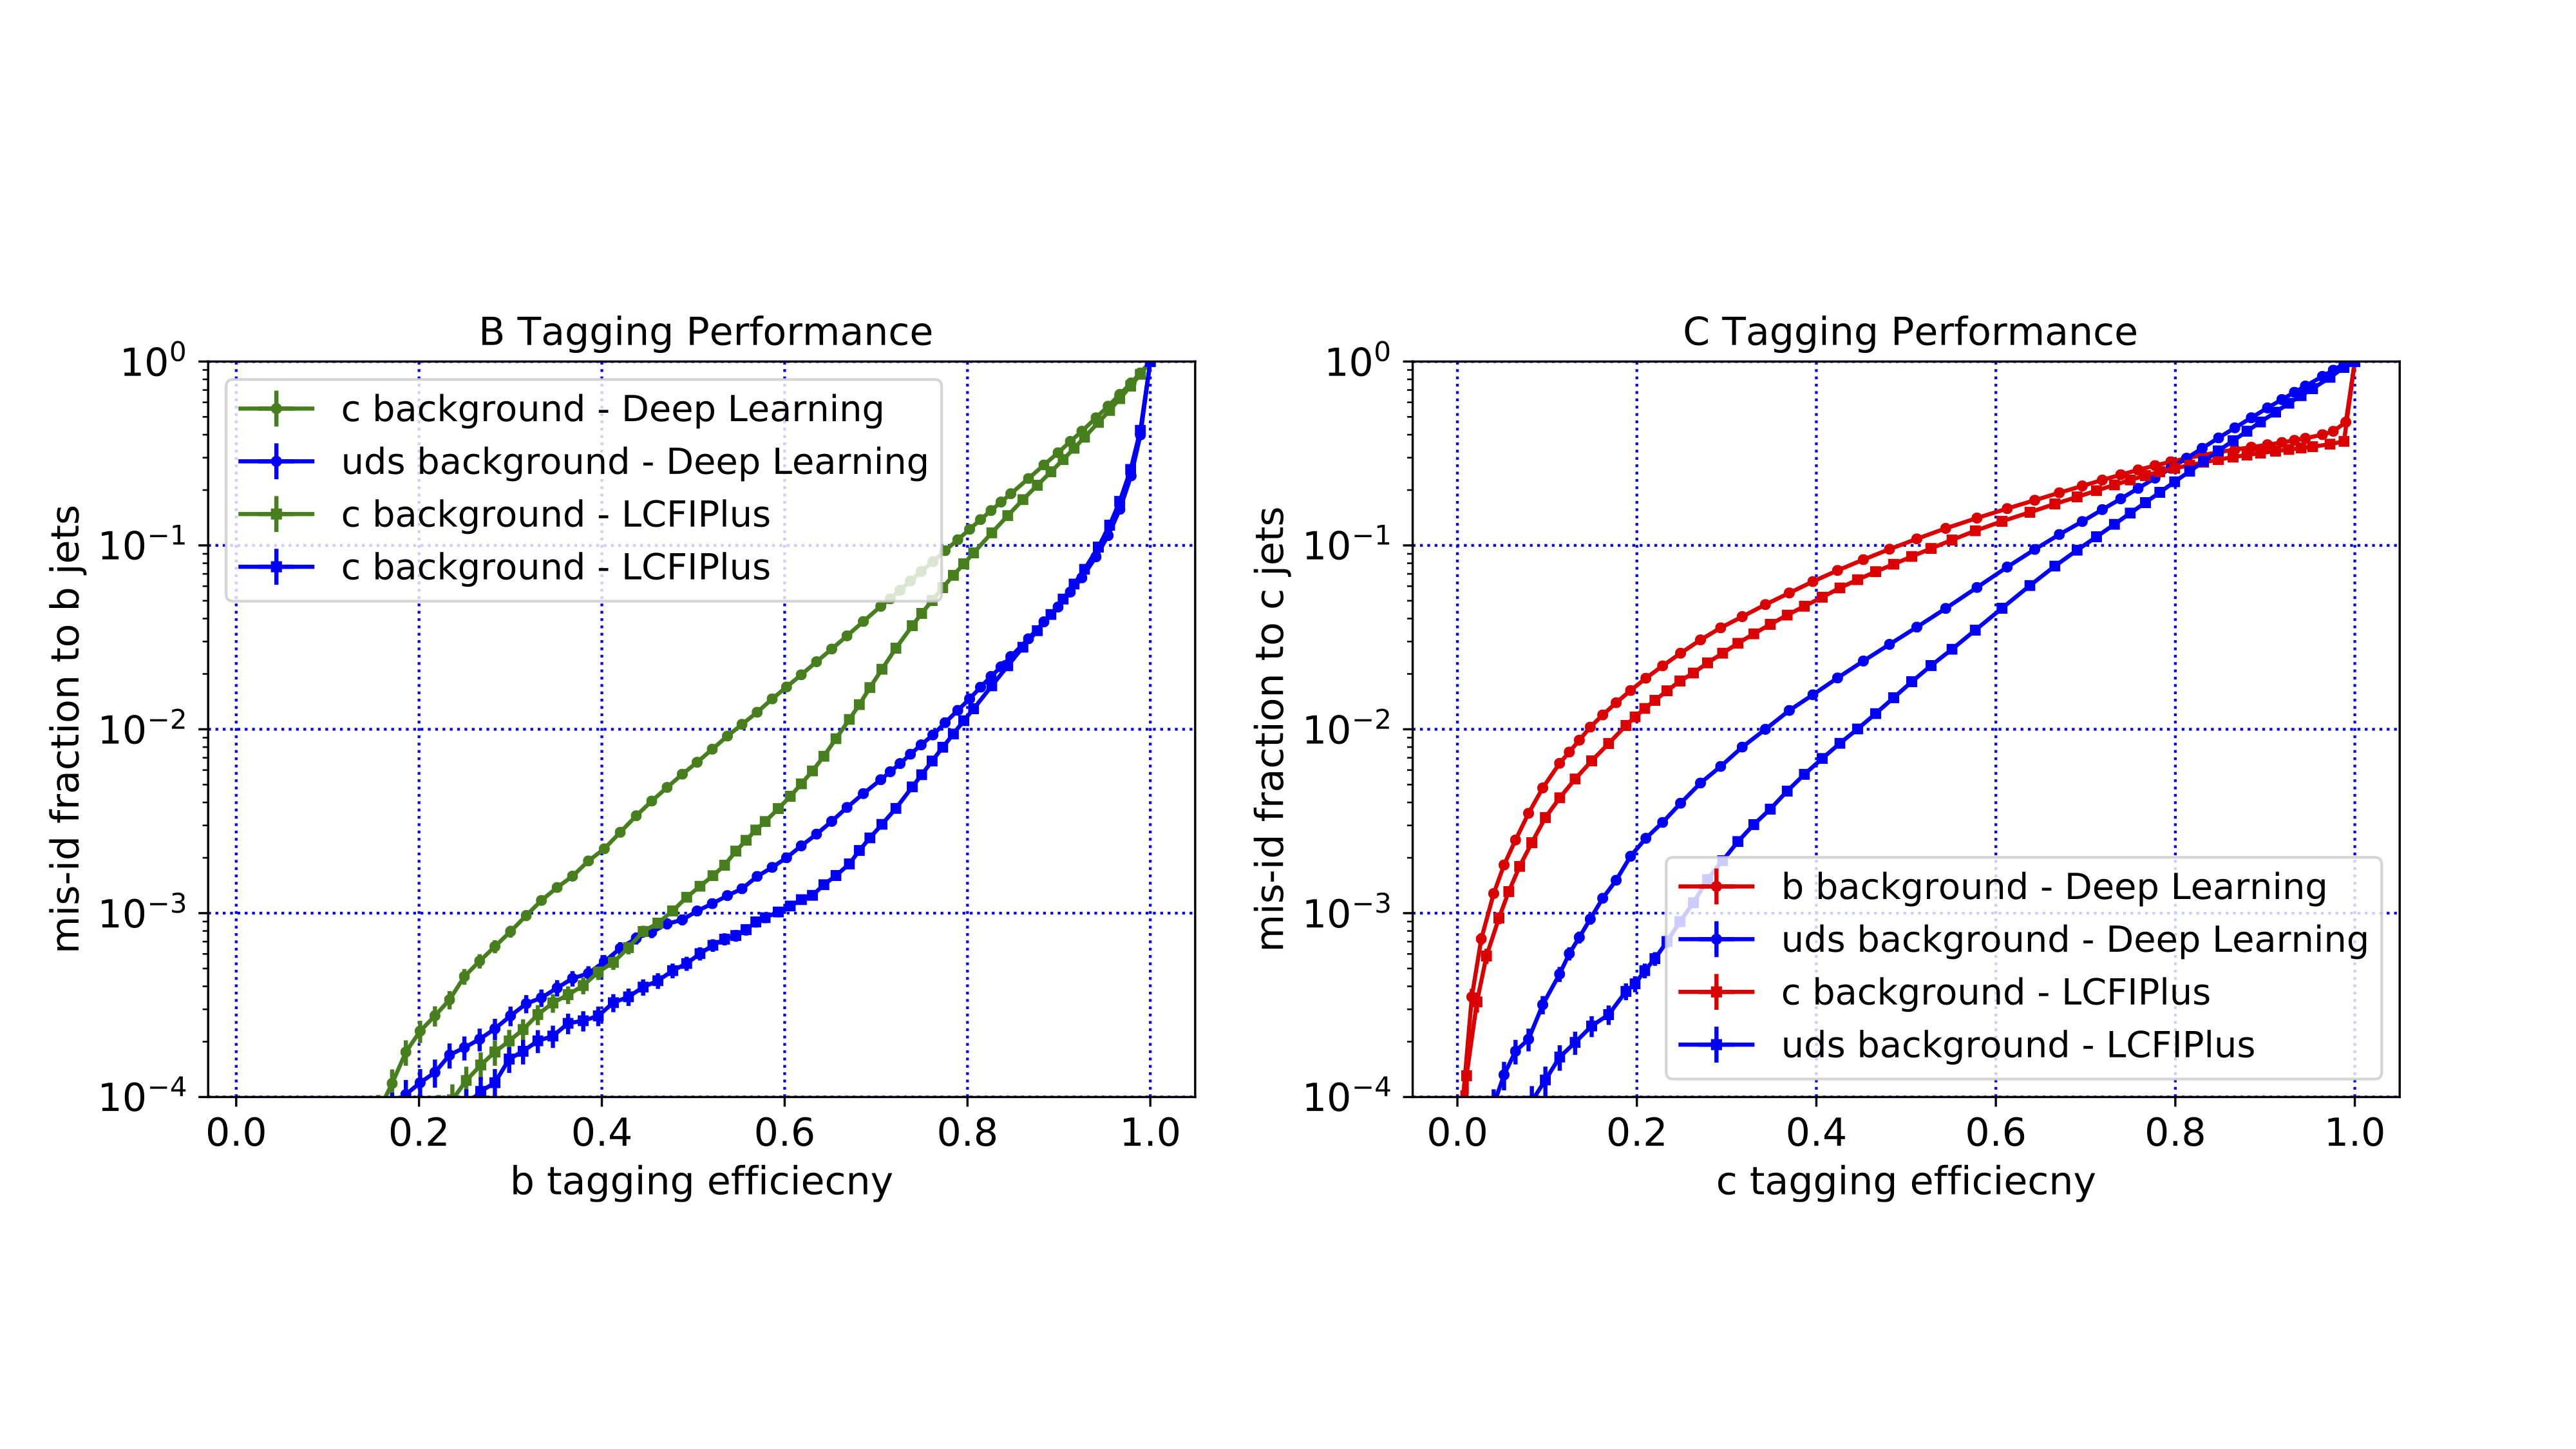
\includegraphics[width=1.0\textwidth, clip]{Figure/5Comparison/5-2-3-1FlavorTaggingROCCurve.png}
 \caption[フレーバータギングの性能に関するROC曲線]{フレーバータギングの性能に関するROC曲線}
 \label{5-2-3-1FlavorTaggingROCCurve}
\end{figure}























